% Inspired by the template by Dave Stevens - https://github.com/davestevens/Loughborough-University-PhD-Thesis-Template/blob/master/thesis.tex
% A4 paper size selected, default is 11pt font, to change to 12pt use [a4paper, 12pt] as option to documentclass
\documentclass[a4paper]{report}

\usepackage{acronym}
\usepackage[dvips]{graphicx}
\usepackage{listings}
\usepackage{color}
\usepackage{url}
\usepackage{fancybox}
\usepackage[includeheadfoot,margin=3.5cm]{geometry}
\usepackage{fancyhdr}
\usepackage{titlesec}
\usepackage{todonotes}
\usepackage{parskip}
\usepackage{biblatex}

\graphicspath{{./images/}}
\addbibresource{references.bib}

\linespread{1.3}

% Setup headers and footers
% \pagestyle{fancy}
% %\fancyhf{}
% %\lhead{\leftmark}
% % Center on all pages
% % \fancyhead[C]{---Draft---}
% % Page number placed on right side on odd pages and left side on even pages
% \fancyfoot{}
% \fancyfoot[LE,RO]{\thepage}
% \fancyfoot[LO,RE]{Tyler Bowcock}


\begin{document}
\pagenumbering{roman}

% Title, Author, Abstract, Acknowledgement, Table of Content, etc....

% Front Page begins

\thispagestyle{empty}

\fancypage{}{\fbox}

%\thisfancyput{%

%Substitute with the right information
\Large{
    \hfill \begin{tabular}{l}
        Computer Science \\
        %Replace this text with your degree name, e.g., Compute Science, Computing and Management, Information Technology and Management of Business, Compute Science and Mathematics, Compute Science and Artificial Intelligence
        COC251 \\
        %e.g COC251, COC252, COC253, COC255, COC257, COC800, COD290 
        B927949
        %Replace this text with your ID number
    \end{tabular}
    }
    
    
    \begin{center}
%\bigskip
%\bigskip
\vspace*{\fill}

%replace by your Project title
\Large{\textbf{Creating a knowledge base \\for The Binding of Isaac}}

\vspace*{\fill}

by

\vspace*{\fill}

%Replace by your name
Tyler J. Bowcock


%Replace by your supervisor's name
\vspace*{\fill}
Supervisor: Dr.\ D D Freydenberger
\vspace*{\fill}

\underline{Department of Computer Science} \\
\underline{Loughborough University}

\vspace*{\fill}
May 2023

\end{center}

% Front Page ends

\newpage

%Reset so that next pages do not have a box around them
\fancypage{}{}


\begin{abstract}
\end{abstract}

\tableofcontents

\addcontentsline{toc}{chapter}{\protect\numberline{List of Acronyms}}
\chapter*{List of Acronyms}
\begin{acronym}
    \acro{HTTP}{Hyper-Text Transfer Protocol}
\end{acronym}

\pagenumbering{arabic}

\chapter{Introduction}
\section{Problem Definition}
Item interactions are an important mechanic of most modern roguelike/roguelite games, including The Binding of Isaac. 
However, with hundreds of items, each with a handful of good or bad interactions, it is nearly impossible to effectively
 remember them all. Graph databases are purpose-built to store and navigate relationships.\cite{WhatGraphDatabase} 
The output of this project will be a web application that leverages this feature of graph databases to allow users to query item 
interactions in The Binding of Isaac.
\section{Aims and Objectives}
The goal of this project is to make querying item interactions in The Binding of Isaac quicker and easier by using graph
 databases. Users will also be able to update the data in the database to ensure it matches any changes in the game.\par
The aims of the project are to:
\begin{enumerate}
    \item Create a graph database containing relevant data about The Binding of Isaac.
    \item Develop a web application that utilises a graph database to helps users to find item interactions in the game.
    \item Explore testing methodologies to aid in producing a stable application with high quality code.
    \item Search for possible ways to extend the project with future updates.
\end{enumerate}
\section{Risks and Constraints}
\subsection*{Cost}
This project has no budget and so any services used in the development of the application will need to be free.
\subsection*{Dataset Availability}
The data needed to create the database may become unavailable or unusable.
\section{Project Plan}
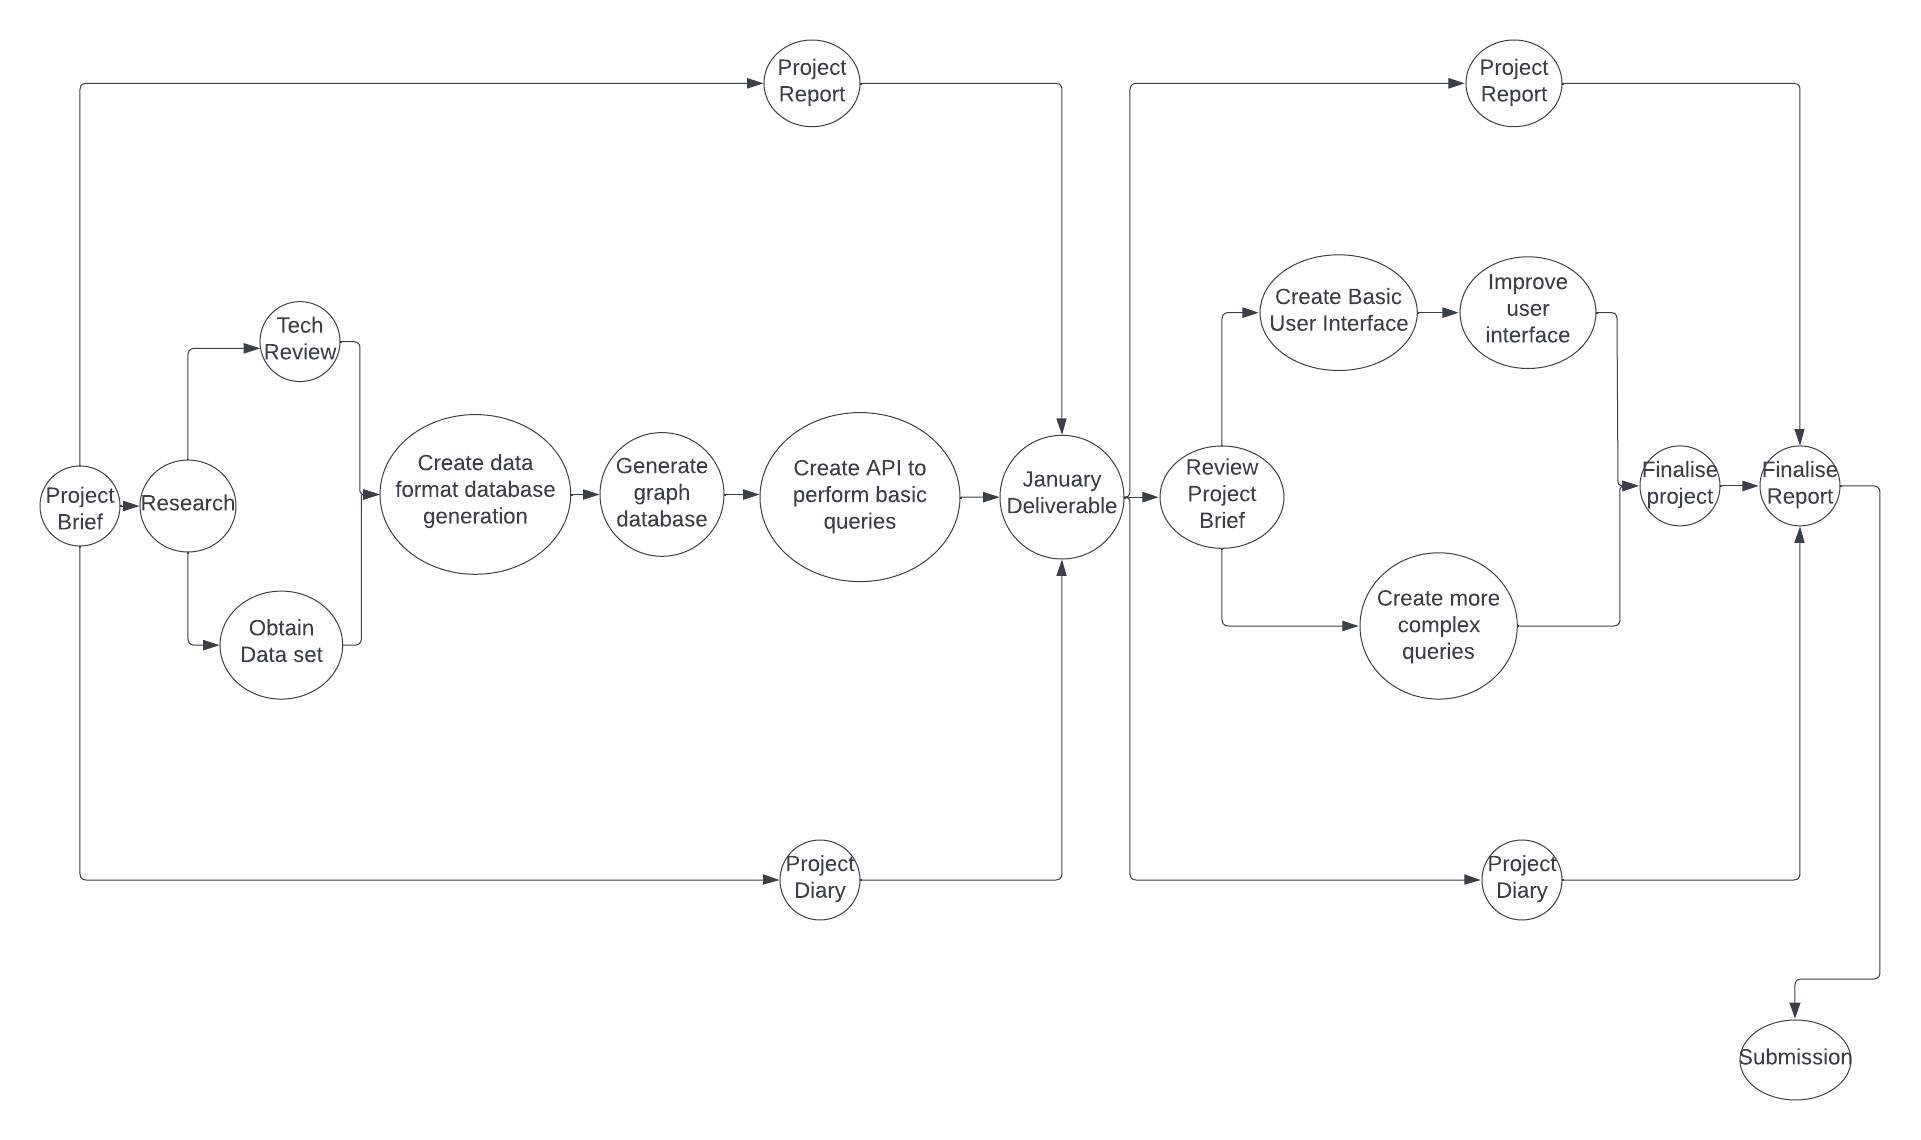
\includegraphics[angle=90,scale=0.7]{PERT}

\chapter{Background}
\section{Introduction}
\section{Existing Solutions}
\subsection*{Fandom Wiki}
\subsection*{Platinmum God}
\section{Technology Review}
\subsection{Database}
\subsection{Client Side Framework}
\subsection{Server Side Framework}
\subsection{Hosting}
\subsubsection*{AWS}
\subsubsection*{Azure}
\subsubsection*{Google Cloud}
\subsection{CI/CD}
\subsubsection*{GitHub}
\subsubsection*{CircleCI}
\subsubsection*{Jenkins}
\section{Conclusion}

\chapter{Requirements}
\section{Introduction}
\section{User Requirements}
\section{System Requirements}
\section{Wireframes}
\section{Conclusion}

\chapter{Design}
\section{Introduction}
\section{System Design}
\begin{figure}[h]
    \centering
    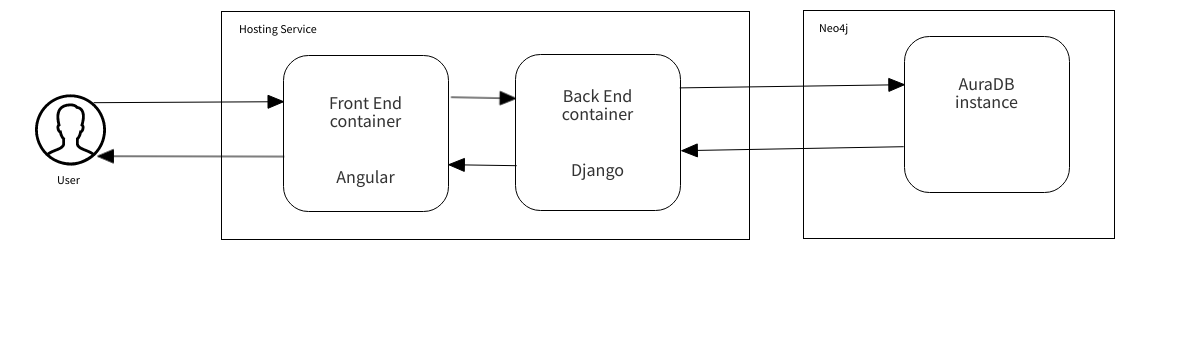
\includegraphics[scale=0.4]{system}
    \caption{System Architecture Diagram}
\end{figure}
The system architecture for this project is similar to most web based applications as the only real difference is the type of database used.
This means the user interacts with the web page created by the front end server, this then communicates with a separate back end server 
using the defined API. If needed the backend server can then communicate with the database, which in this case is hosted 
remotely by Neo4j.
The front and back end servers would likely be hosted in the cloud via the use of some containerisation system such as Docker.
\section{UI Design}
Given that the data is stored in a graph database and that is the focus of this project, it seemed obvious to display the data 
to the user as a graph. This idea was further reinforced by looking at the Neo4j tool Bloom. As shown in the screenshots below, 
Bloom is used to display the data in a dynamic and responsive graph. The main view area is called the "Scene" and just this alone allows 
the user to quickly visualise the data and see the relationships formed. In the scene the nodes can be dragged using the mouse and the graph updates 
using a physics simulation to move the other nodes. This helps ensure the other areas of the graph are still readable while still allowing the 
user to manipulate the graph.
\begin{figure}[H]
    \centering
    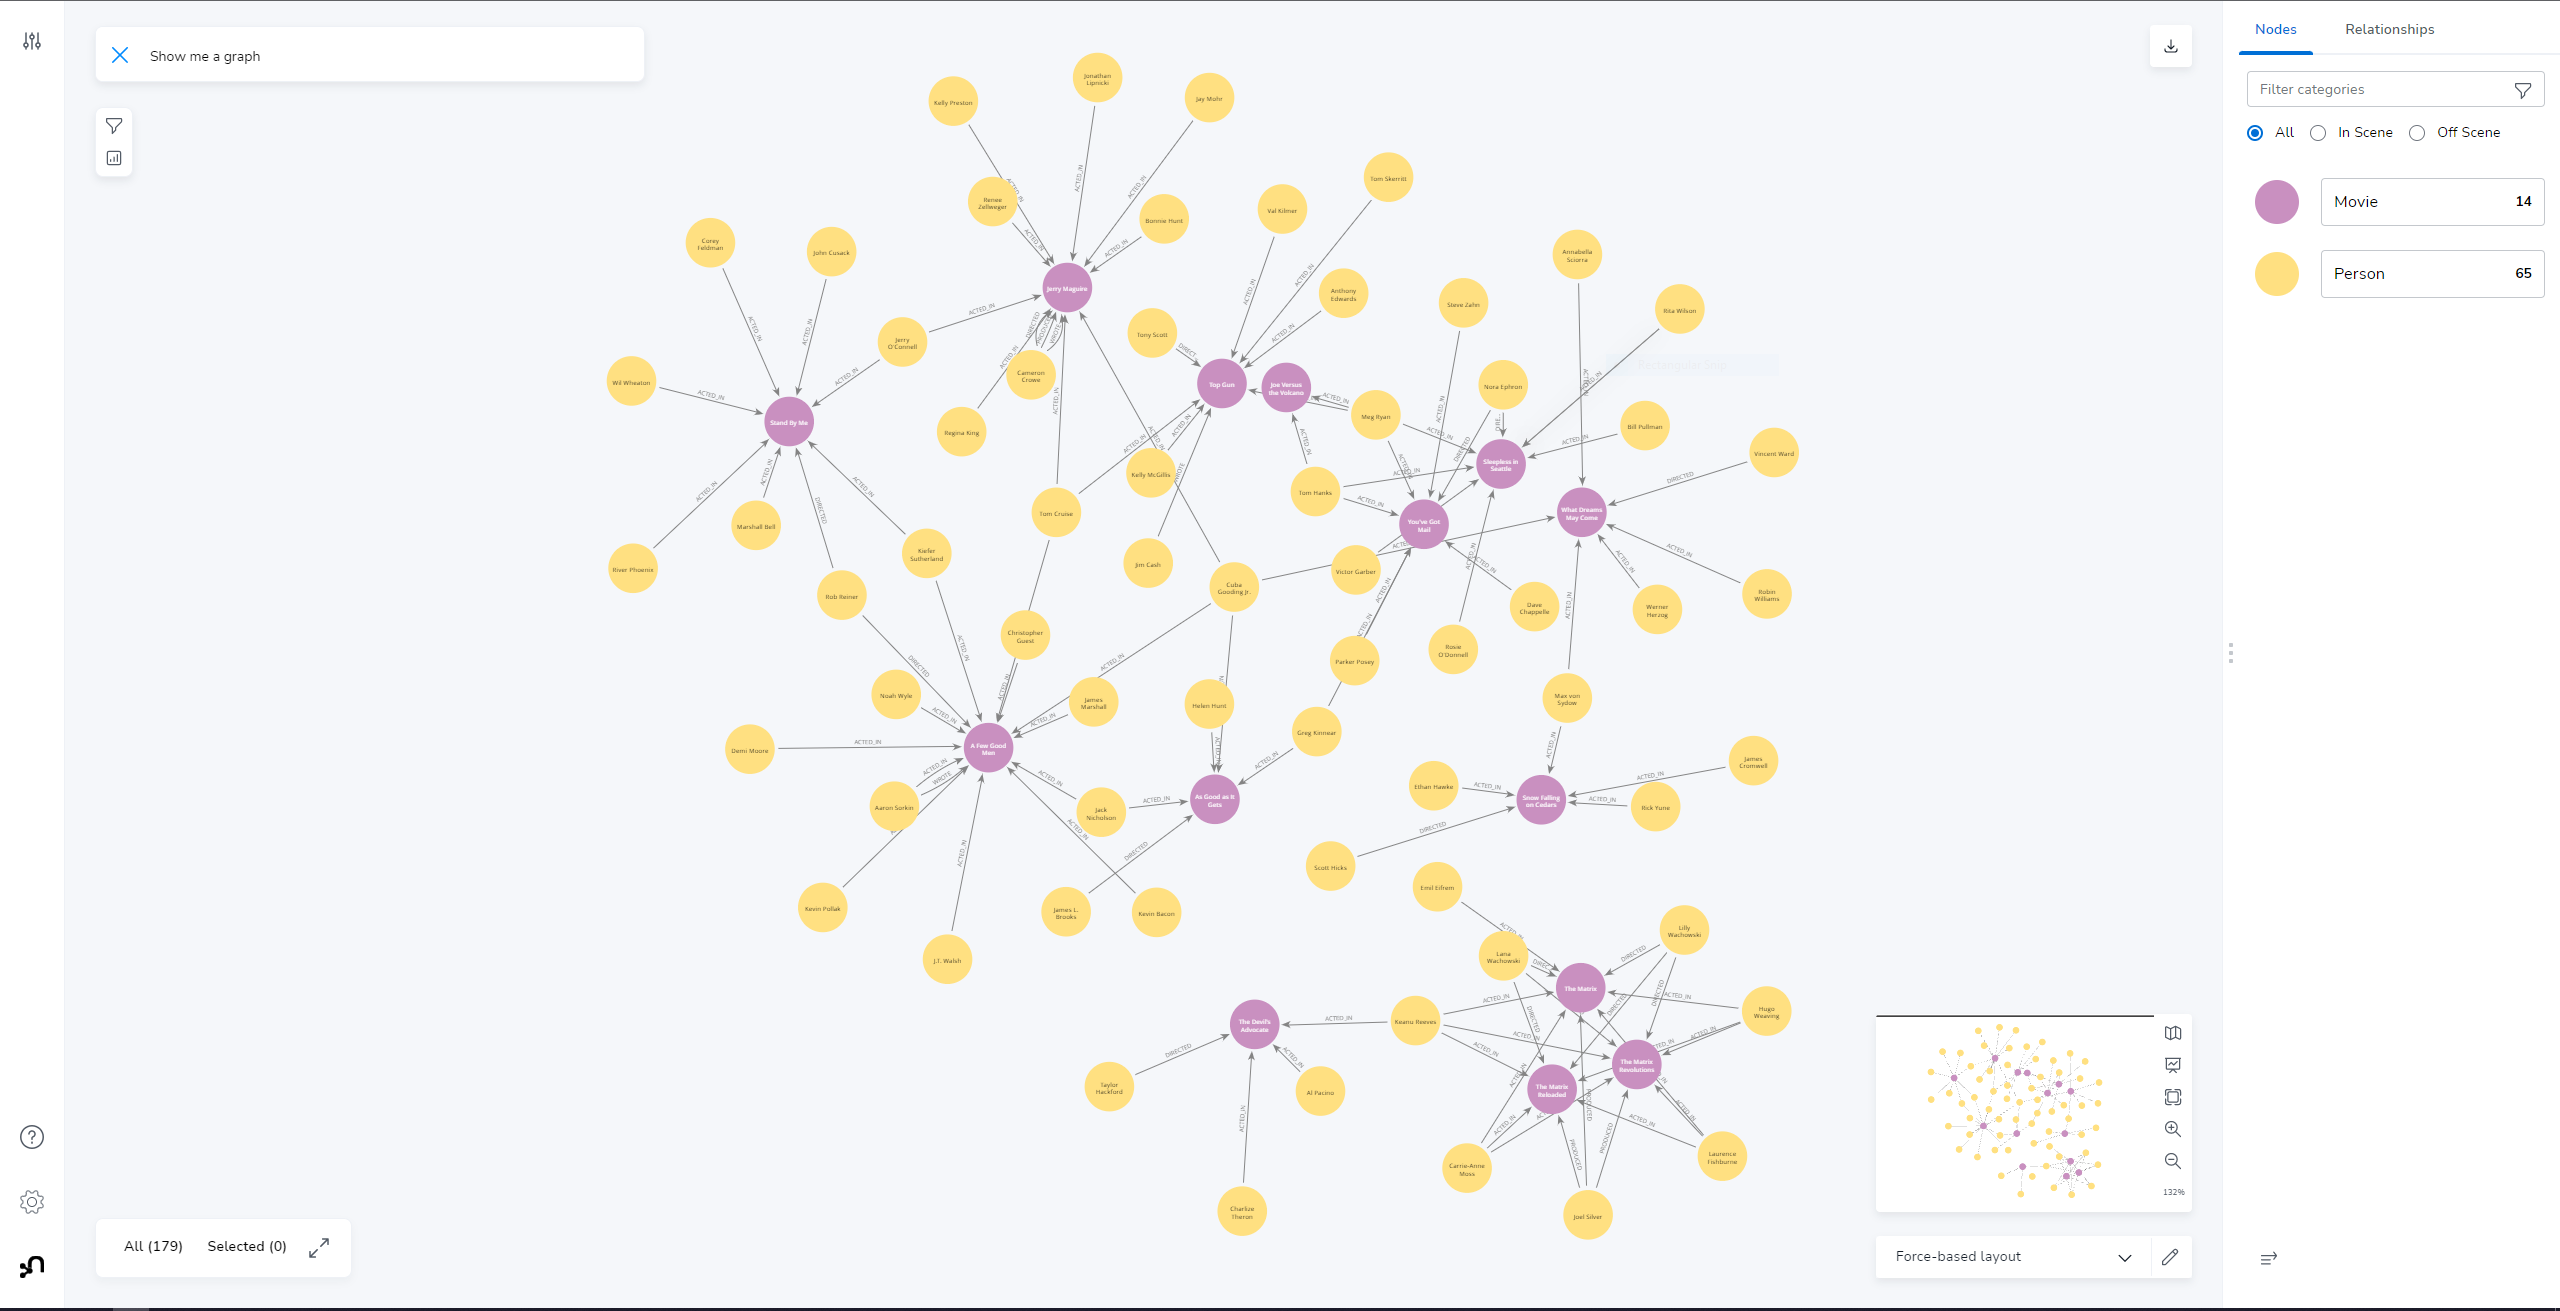
\includegraphics[width=0.8\textwidth]{bloomExample}
    \caption{Neo4j Bloom using the demo Movies database}
\end{figure}
Figure 3.3 shows two key features of Bloom. The first is the `inspect' element which allows the user to view the full properties 
of a node or relationship by double-clicking them. This means the graph itself is not cluttered with extra information but the user can 
still easily access that data when required. The other feature is the search bar which has a few unique functions that utilise the 
graph structure of the database. It uses the types of nodes and relationships in the database to provide some quick pre-filled searches, 
For example Actor - ACTED\_IN - Movie with the demo database. This can be used to quickly filter out unwanted data from the scene without having to know 
how to write custom query statements. The second functionality follows on from this, in that the user can define their own query statements which 
become a command available in the search dropdown. This is useful if the user is familiar with Neo4j's own query language CYPHER, and they want 
to leverage that for more powerful querying.
\begin{figure}[H]%
    \centering
    \subfloat[\centering Bloom Inspect Element]{{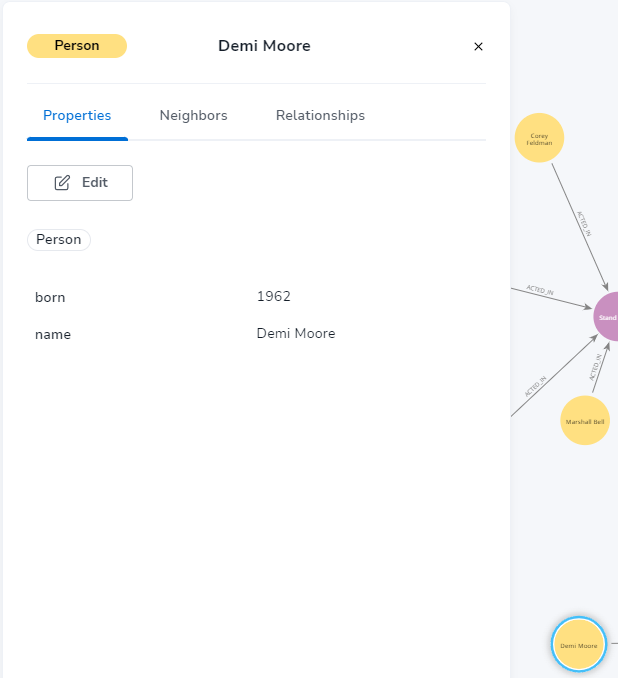
\includegraphics[width=0.4\textwidth]{images/bloomInspect.png}}}%
    \qquad
    \subfloat[\centering Bloom Search Element]{{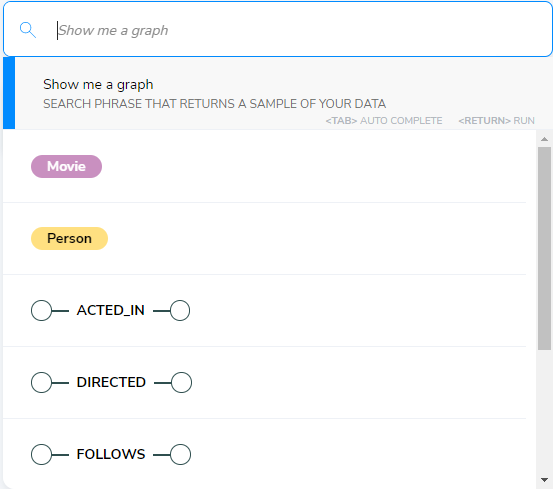
\includegraphics[width=0.4\textwidth]{images/bloomSearch.png}}}%
    \caption{Neo4j Bloom inspect and search elements}
\end{figure}
These are all features that should be considered when implementing the user interface, however not all of them are essential for a usable application.
\section{Conclusion}

\chapter{Implementation}
\section{Introduction}
\section{Tools}
\subsection{IDE}
Visual Studio Code was used for this project due to prior experience with the IDE. It is also one of the most popular tools in the industry 
as shown by the Stack Overflow Developer Survey\cite{StackOverflowDeveloper} and the TOP IDE Index\cite{TOPIDETop}.
VS Code has excellent support for many programming languages, and with a wealth of community made extensions there are many tools to aid with development.
\subsection{Version Control}
Version control is a system that records changes to a file or set of files over time so that you can recall specific versions later.\cite{GitVersionControl}
Using version control with an external hosting provider also makes working over several computers easy which will be useful for this project, and it ensures everything is backed up remotely.
Git was chosen for version control as it is the industry standard, with GitHub being used as the hosting provider.
\subsection{Database Visualisation}
Neo4j has two tools for database visualisation as part of the AuraDB web interface; Bloom and Browser. Bloom is used to 
visualise the data in a graph as has been discussed in the design chapter previously. Browser is used to test CYPHER queries on the database.
CYPHER is the query language created by Neo4j for retrieving data from their graph databases. As shown Figure 4.1, the user can enter a 
query and have the data returned as a graph, table (represented as a series of JSON objects), raw text and as code (JSON objects).
This is useful for quickly testing CYPHER queries and debugging database interactions.
\begin{figure}[h]
    \centering
    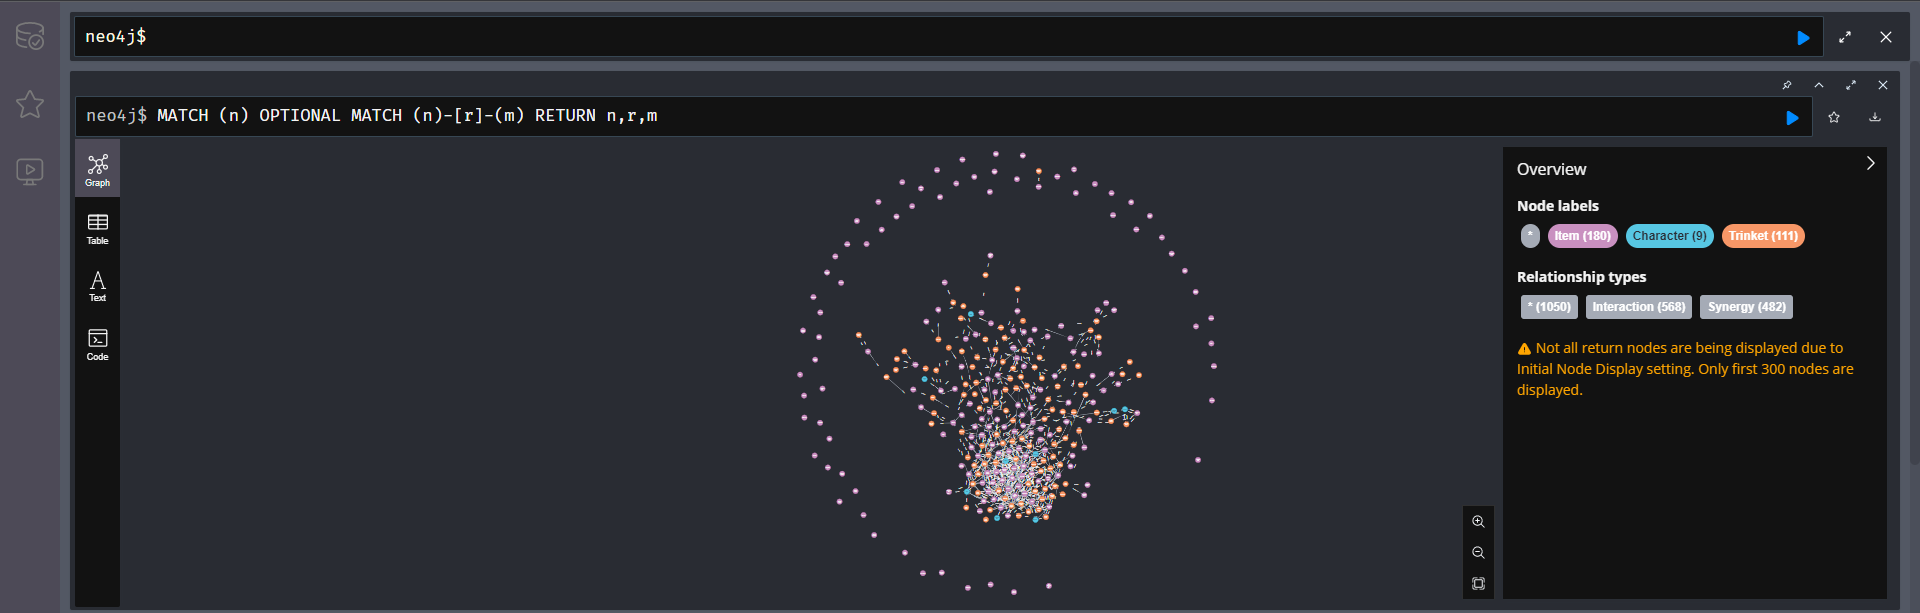
\includegraphics[width=0.8\textwidth]{neo4jBrowser}
    \caption{AuraDB Browser}
\end{figure}
\section{Libraries}
\subsection{Data Processing}
\begin{description}
    \item[Beautiful Soup] - A Python library for pulling data out of HTML and XML files\cite{BeautifulSoupDocumentation}. 
    Used to parse the XML dump and extract data for the database.
\end{description}
\subsection{Client Side}
\begin{description}
    \item[Cytoscape] - A JavaScript library that `allows you to easily display and manipulate rich, interactive graphs'\cite{franzCytoscapeJsGraph2016}. 
    Used in this project to display the data in graphs to the user.
    \item[Material] - An Angular specific library containing material design components, used in this project to quickly create UI components.
\end{description}
\subsection{Server Side}
\begin{description}
    \item[Neomodel] - An Object Graph Mapper (OGM) for the Neo4j graph database\cite{NeomodelDocumentationNeomodel}, used to define Django models for access database data.
    \item[django-cors-headers] - A Django App that adds Cross-Origin Resource Sharing (CORS) headers to responses. This allows in-browser requests to your Django application from other origins.\cite{yiuDjangocorsheadersDjangocorsheadersDjango} 
    this is required for the front end and back end to communicate properly.
\end{description}
\section{Data Processing}
The first major section of the implementation was setting up the graph database and getting the data required to do so.
\subsection{Finding Data Source}
The initial project brief suggested using the Fandom wiki for the data source as Fandom wikis have the option for downloading 
an XML dump from the \verb|Special:Statistics| page. As discussed in section 2.3, the Fandom wiki is also the most comprehensive 
source of data about the game, especially regarding the item interactions. The XML dumps are not always kept up to date, so while 
a new dump was being requested other options for the data source were investigated. This included investigating the game files, where 
all the resource files have been packed in to \verb|A| files. In the folder containing the resource files there is a readme which explains 
that this was done to prevent spoilers and any secrets being found through the files. A resource extractor tool is included with later versions of the game, 
however the files do not contain any information regarding the interactions of items.\par
Once received, the updated XML dump presented its own challenges, the first being its size, at just under 500,000 lines long and around 20MB it was too 
large for most text editors to load with syntax highlighting. This made it difficult to understand the structure of the data as the XML tags became harder 
to pick out from regular text. Aside from a small preamble, all the data in the file is contained in a series of \verb|page| elements, which unsurprisingly represents a page on the site.
Each page element has a similar structure to the below example (Fig. 4.2).
\begin{figure}[H]
    \begin{lstlisting}[language=XML]
        <page>
        <title>Template:</title>
        <ns>10</ns>
        <id>161</id>
        <redirect title="Template:*" />
        <revision>
          <id>161</id>
          <timestamp>2014-09-16T20:27:12Z</timestamp>
          <contributor>
            <username>Maintenance script-gpuser</username>
            <id>41555837</id>
          </contributor>
          <comment>&amp;lt;default import&amp;gt;</comment>
          <origin>161</origin>
          <model>wikitext</model>
          <format>text/x-wiki</format>
          <text bytes="24" sha1="2dwqfi7oey6311xkwxu3dhjasn8gfsi" xml:space="preserve">#redirect [[Template:*]]</text>
          <sha1>2dwqfi7oey6311xkwxu3dhjasn8gfsi</sha1>
        </revision>
      </page>
    \end{lstlisting}
    \caption{Example page format}
\end{figure}

The important parts to note from this is that the \verb|title| element is the web page title and the \verb|text| element contains the data to be displayed (or in this case a redirect to another page).
There doesn't appear to be a particular order to the pages and due to the formatting of the file it can be hard to tell where one page ends and another begins.
\subsection{Data Extraction}
Due to the structure of the XML data, the easiest way to extract the data is to use the title tags for each page to find the relevant and pages 
and then pull the data from the text tag. The XML file contains collections pages which each contain a list of items available in each version of the game, this can be 
used to get a list of all the item names. Character names are fetched from the \verb|Characters| page. This has a list of links to the character pages, from which the names can be extracted using RegEx. 
Unfortunately, the same does not exist for trinkets as the page that would contain that list instead uses a template which autofills the data. 
As a temporary fix, the list of trinkets is fetched from a hardcoded file.
\begin{figure}[H]
    \begin{lstlisting}[language=Python]
        ITEM_REGEX = re.compile("content =(.*?)}}", flags=re.DOTALL)

        def _get_item_names(self):
            collection = self.soup.find("title", text="Collection Page (Repentance)").find_parent("page").find("text").text
            return [
                x.strip()
                for x in ITEM_REGEX.search(collection)[1].replace("\n", "").replace("Number Two", "No. 2").split(",")
            ]
    \end{lstlisting}
    \caption{Function that returns the list of item names}
\end{figure}

Figure 4.3 shows the code used for getting the list of item names, similar code has been used for getting character names.
\verb|re| is a Python library that provides regular expression matching operations. In the data extraction script a series of 
compiled RegEx statements are defined as constants, \verb|ITEM_REGEX| being one of them. These are used through the script 
to pull data from the XML file based on the format of the data. Here BeautifulSoup is used to find the title tag that contains the text 
`Collection Page (Repentance)', this is then used to get its parent and to search that for the text element. 
To get the data from the string of text the RegEx statement is used to search for a string that starts with \verb|content =| and ends with \verb|}}|.
The \verb|(.*?)| matches a string of any characters of any length non-greedily and puts it in a match group. 
This means it will match against any character until the first instance of \verb|}}| and the object returned is sub-scriptable to get the match groups.
Accessing group 0 is the whole match which will included the \verb|content =| and \verb|}}|, accessing group 1 is the first (and in this case only) match group.
The string returned by accessing the match group then has new line characters removed and and is split into a list using the commas.
Each value in this array then has any leading and trailing whitespace removed using \verb|strip()| and a list comprehension.
There is an extra step needed here due to the nature of the XML data and that is manually replacing the item name for `Number Two'.
This had to be done as the name appears in several formats throughout the data, but the only one that has a page with data in is `No. 2'. 
The rest of the pages just redirect back to that page and so instead of handling the redirect it is easier to catch and replace the different formats when they appear.

Functions could now be written for getting item, trinket and character data respectively. These functions all follow the same format 
and the differences are in catching special exceptions and the output created.
\begin{figure}[H]
    \begin{lstlisting}[language=Python]
        def get_all_items(self) -> list:
        item_names = self._get_item_names()
        tags = self.soup.find_all("title")
        item_data = []
        for tag in tags:
            if tag.text not in item_names:
                continue

            item_text = tag.find_parent("page").find("text").text

            item_id = self._infobox_get(item_text, ID_REGEX)
            if item_id is None:
                continue

            item_data.append(
                [
                    tag.text,
                    f"I{item_id}",
                    self._infobox_get(item_text, QUOTE_REGEX),
                    self._infobox_get(item_text, DESCRIPTION_REGEX),
                    self._infobox_get(item_text, ITEM_QUALITY_REGEX),
                    self._infobox_get(item_text, UNLOCK_REGEX),
                    self._list_get(item_text, EFFECTS_REGEX, True),
                    self._list_get(item_text, NOTES_REGEX, True),
                ]
            )
            self.id_lookup[tag.text.lower()] = f"I{item_id}"
            self.synergies[tag.text] = self._list_get(item_text, SYNERGIES_REGEX)
            self.interactions[tag.text] = self._list_get(item_text, INTERACTIONS_REGEX)
        return item_data
    \end{lstlisting}
    \caption{Function that extracts the item data}
\end{figure}
Each function iterates over the title tags in the XML file and checks if it is in the list of tags being looked for. 
If it is the text element belonging to that title tag is fetched and an attempt at getting the item ID is made. This is done 
by passing the relevant compiled RegEx statement and the text to process to a function which will execute the RegEx and return \verb|None| 
if no match is found and the ID string if a match is found. If no ID is found that means the page found isn't actually an item page and so can be ignored.
The rest of the data can then be extracted using the same method as for getting the ID, the only difference being for the effects and notes data another function 
is used that has extra processing for handling lists in the text. The synergy and interaction data is added to a separate dictionary as it requires extra processing 
to create usable data. The item name and ID is added to a lookup dictionary which will be used later when processing the synergies/interactions.
Importantly, for each ID a letter prefix is added to indicate whether the ID belongs to an item, trinket or character; this is needed to ensure the IDs 
are unique across the entire database.

The function for getting character data is much simpler than for items and trinkets, this is because it only gets the character name and ID. 
The decision was made to ignore character data because it is much more complicated than any of the other data types. The page for each character has 
a unique structure, especially for characters that are a combination of two characters such as Jacob and Esau or The Forgotten. Combined with the fact that 
most of the character data does not contribute to the relationships in the database which is the main focus, it was decided that processing the character data was outside 
the scope of this project. 

Once all the item, character, and trinket data has been extracted the lookup dictionaries can be used to process the synergies and interactions. 
The function to process the data is fairly simple, it iterates over each entry in the dictionary, each entry contains a list of strings. That list is iterated over 
and the RegEx show in figure 4.5 is applied to create a list of item names which represent the relationship destination. The RegEx looks for tags that link to other items/characters/trinkets,
for example {{i|Libra}}. However, these tags don't seem to always follow a set structure which is why the RegEx has some extra match groups either side of the \verb|(.+?)| group to catch and ignore extra 
characters that are not relevant. These irregularities also mean an if block is needed to catch links where the link text does not match the text in the title tag.
\begin{figure}[H]
    \begin{lstlisting}[language=Python]
        destinations = re.findall(r"{{[ict]\|(1=)?(.+?)(\|.+?)?}}", relationship[0], re.IGNORECASE)
    \end{lstlisting}
    \caption{Synergy/Interaction RegEx}
\end{figure}
The ID lookups are then used to find the ID for the source entity and the destination entity found via the RegEx. This is then added to the output along with the string containing the relationship data.
\subsection{Cleaning the Data}
The data extracted above still contains special characters and formatting that is used by the XML to generate the website correctly. 
This includes \verb|<br>| HTML tags, tags using square brackets to denote alternative text/images and the curly brace tags seen above which are used for a variety of purposes.
One of the uses of curly brace tags is to show which version of the game the information is relevant to; on the webpage this is show via a small image but in the XML
that image is represent by a tag in the following format \verb#{{dlc|<tag>}}# where \verb|<tag>| is replaced by a code that represent the game version.
These tags are replaced with a relevant string using RegEx, e.g. \verb#{{dlc|anr}}# becomes `(Added in Afterbirth, Removed in Repentance)'.
RegEx is then used to extract the useful text from the rest of the tags and remove the brackets and any other formatting characters.

The lists used when processing synergies and interactions have to be generated from the string return by the data extraction.
In the XML the bullet pointed lists are represented using `*' characters where the number of characters indicates the level of indentation.
The string is split using the bullet characters and then a recursive function is used to create a nested list that represents the list indentation.
Optionally, the function can also take the nested list and create a formatted string with tab spacing to create the indentation.
\subsection{Importing into Database}
The AuraDB platform provided by Neo4j has a data importer tool which uses CSV files to populate a predefined model. 
Creating CSV files with Python is very simple, the data needs to be in a 2D array where each inner array is a row in the CSV file,
the CSV writer also takes a list of headers and from the two it can create a CSV file. The CSV files needed to be created so that each file represents 
a node/edge in the model, this meant 5 CSV files were needed. With the files uploaded to the import tool the model shown in figure 4.6 could be created.
\begin{figure}[H]
    \centering
    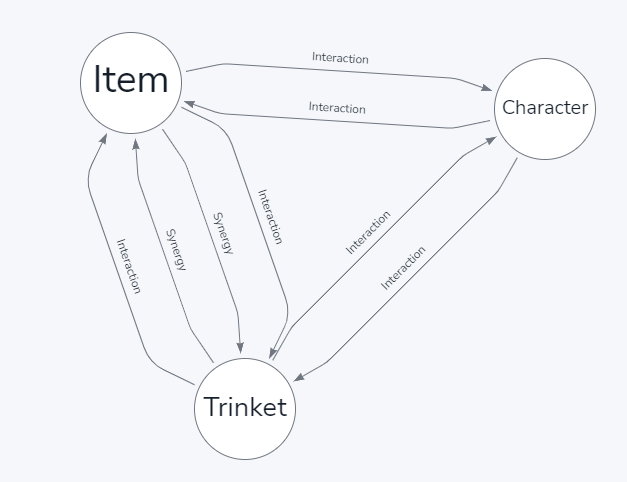
\includegraphics[scale=0.3]{dataImport}
    \caption{Database Model in Neo4j Data Importer}
\end{figure}
As the model shows items and trinkets can have interactions and relationships between each other and themselves. The relationships to character 
entities are only towards the character nodes because the character data is not processed as discussed above.
After importing the data Neo4j Bloom can be used to check the database structure which is show in figure 4.
\begin{figure}[H]
    \centering
    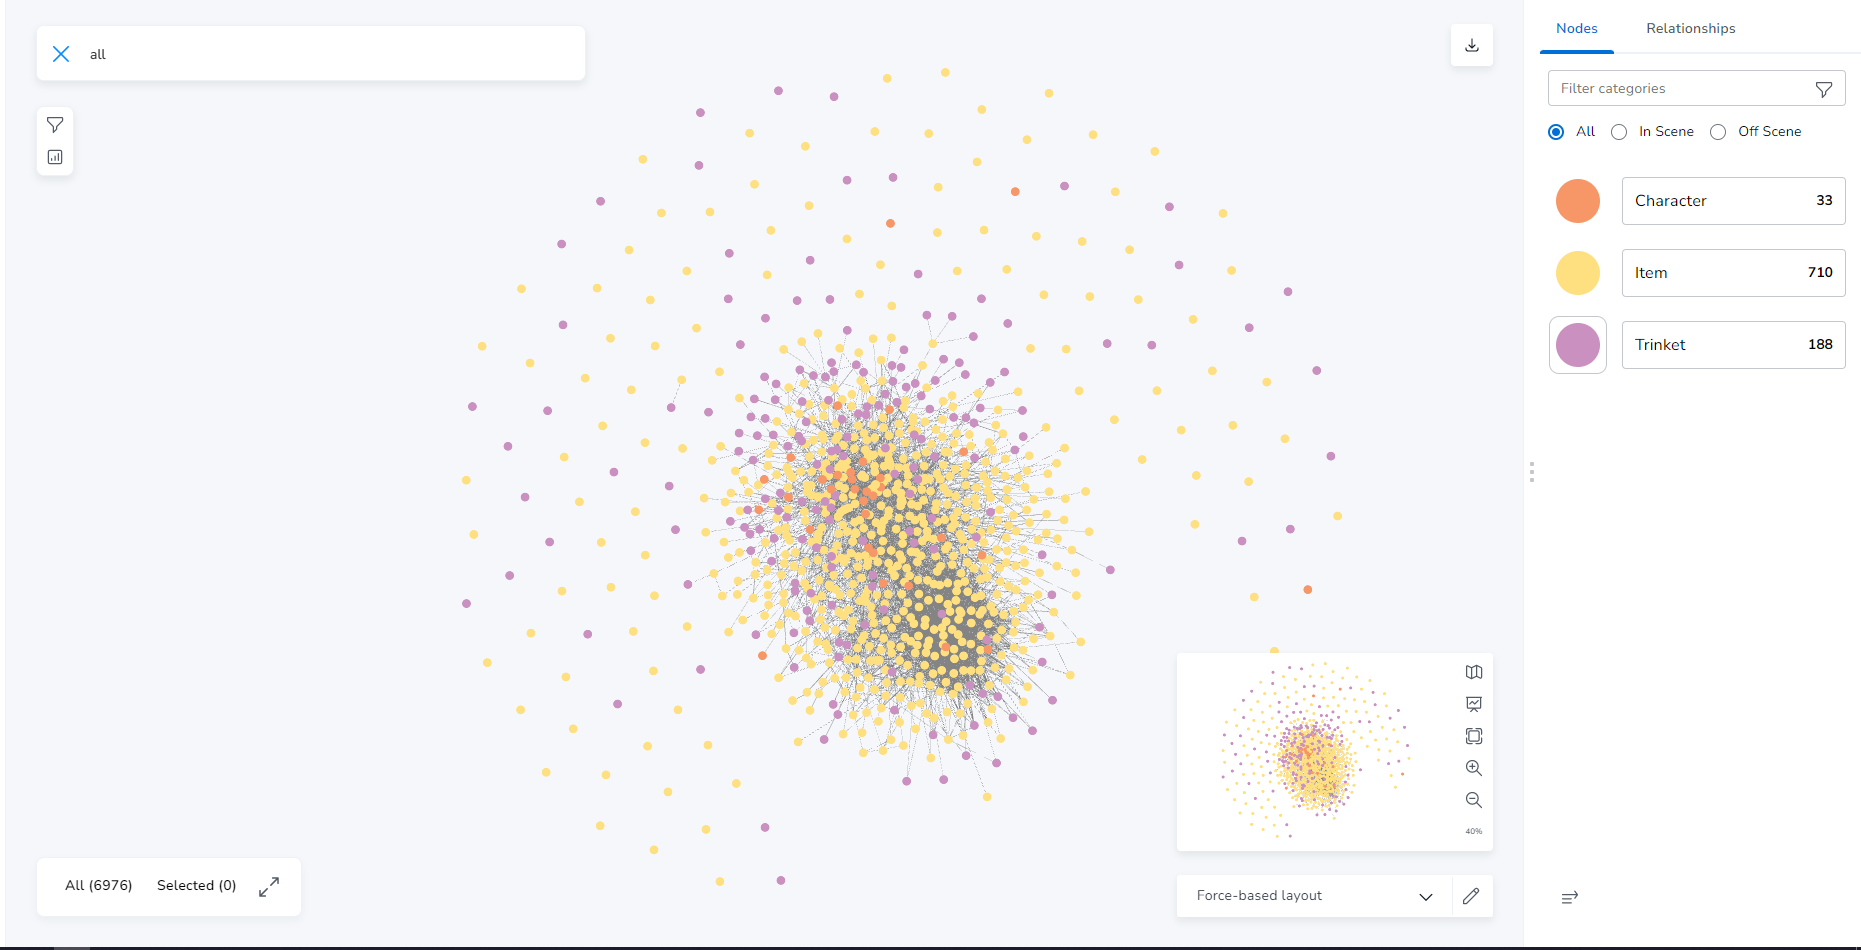
\includegraphics[width=0.8\textwidth]{importedData}
    \caption{Bloom showing complete database}
\end{figure}
\section{Web Stack}
Before the database can be utilised the Angular and Django projects need to be set up and connected to form the web stack.
The first step is to create a Django project, this is achieved using a single command provided by the Django Python library. 
This command creates the base folder structure for the project which includes the management file, an SQL database and several configuration files.
The \verb|manage.py| file is used to perform most admin actions, commonly this is keeping the database migrations up to date and running the web server; 
in this project only the latter is needed due to using a different database. Out of the configuration files generated, \verb|settings.py| 
is the only one that needs configuring at this stage. Cross-Origin Resource Sharing (CORS) is an HTTP-header based mechanism that allows a server to 
indicate any origins (domain, scheme, or port) other than its own from which a browser should permit loading resources.\cite{CrossOriginResourceSharing2023}
This needs enabling on this project so that the Angular app can send requests to the Django web server from another domain. Enabling CORS headers in Django 
requires the installation of the django-cors-headers Python library and some additional some entries in the \verb|settings.py| file. 
Now a Django app can be created in the project using a command similar to the one that created the project. The app folder contains the models, views and URLs files 
that will contain all the functionality of the backend. \verb|models.py| is the where the database interaction is defined, usually this is done via model classes 
and serialisers supplied by Django. However, due to using a database hosted by Neo4j this will be accomplished using the neomodel Python library. 
The \verb|views.py| file sits on top of the models file, it contains the functions that take in HTTP requests, perform some action which may involve using the models 
to interact with the database, and then generate a response. These functions are called by the paths declared in the \verb|urls.py| file, each path defines a URL pattern 
and the view function that should be called to handle it. Some final changes need to be made to the configuration files to finishing setting up the Django app and then the 
backend is ready for development. The first change is to add some paths to the \verb|urls.py| in the main project folder, this is to set which URLs should be directed 
to the app that has just been defined. The other changes are in the \verb|settings.py| file and simply involve including the new app name in the \verb|INSTALLED_APPS| 
section.
\begin{figure}[H]
    \dirtree{%
    .1 DjangoAPI.
    .2 DjangoAPI.
    .3 asgi.py.
    .3 settings.py.
    .3 urls.py.
    .3 wsgi.py.
    .2 QueryApp.
    .3 admin.py.
    .3 apps.py.
    .3 models.py.
    .3 tests.py.
    .3 urls.py.
    .3 views.py.
    .2 manage.py.
    }
    \caption{Folder structure after creating Django project}
\end{figure}

Creating the Angular project follows a similar set of steps to creating the Django project. First a new project is creating using a command 
provided by the Angular library, this creates quite a large folder structure which can be very overwhelming. However, only a handful of these files 
are used over the course of the project. Before configuring any of these, the app components and services need to be created, this is again done using commands provided 
by Angular which generates the following folder structure for each component.
\begin{figure}[H]
    \dirtree{%
    .1 example.
    .2 example.component.css.
    .2 example.component.html.
    .2 example.component.spec.ts.
    .3 example.component.ts
    .3 example.service.spec.ts.
    .3 exmaple.service.ts.
    }
    \caption{Example component folder structure}
\end{figure}
Each component has a structure similar to a normal HTML/CSS/JavaScript application, the exception being TypeScript is used instead of JavaScript.
The additional component file (example.component.spec.ts) is where unit tests should be written, and it includes some basic test structs as part of the 
file generation. \verb|service.ts| files contain classes and functions dedicated to interacting with the back end, for this project there is a shared services file at 
the app level and then each component has a service which inherits from the shared one. Services also have \verb|spec.ts| file for API unit tests.
A final commonly used file type is an interfaces file, this is a regular TypeScript file that contains many interface objects which are exported. 
These are used to define custom data types/objects which are needed as TypeScript is a typed language and the data the front end receives can be in many formats.
Once the components have been created it's important to update \verb|app.module.ts|, this file defines the root module and its contents. 
If a component, service or imported library is not correctly defined in this file, then the project will fail to compile as it will not be able to find all the files required.
Next \verb|app-routing.module.ts| will need configuring, similar to the \verb|urls.py| files in Django, this defines routes as a path and which component should be called for that path.
This information is then used in the \verb|app.component.html| via the \verb|<router-outlet>| element, which will contain the HTML of the corresponding component for the current URL.
The HTML file can also contain HTML elements that are to be displayed across all pages, such as a navigation bar.
The final file of interest is \verb|tsconfig.json|, which is a configuration file that contains compiler options. This often will not require any changes, however 
sometimes it is useful to disable compiler errors, especially when working with third party libraries.

Finally, to connect the Angular and Django project to allow requests and responses to be sent between them, a read only constant is defined 
in the shared service of the Angular component. This constant contains the IP address of the web server created by the Django project, it can then 
be used later when performing HTTP requests to direct them to the back end.
\subsection{Database Interaction}
Neomodel was used to allow Django to connect to the remote database. The username, password and database URI are stored as 
constants which are passed into the neomodel configuration. Then classes can be defined which represent each of the node and edge types.
For node classes, class attributes are defined for each property of the node and for each relationship type the node can have. The relationships 
only need to be defined in one direction and so most of the relationships are defined in the \verb|Item| class. The edge classes only need to 
define the properties of the relationship. These classes contain built-in methods for performing simple queries on the data, for more 
advanced queries neomodel has a method for querying with user defined CYPHER queries.
\subsection{Displaying Data in Tables}
To help ensure the database was functioning properly and to provide an opportunity to learn the intricacies of neomodel in a simpler 
environment, the decision was made to implement displaying the data in tables first. This would require fetching all the data for each 
node and edge type and formatting it correctly. Getting all the data for a set of nodes is easy with neomodel due to the \verb|nodes.all()| method, 
which returns a list of all the nodes for the given node type. However, this data was not in a format accepted by the front end. The list contained 
instances of the model class which have string representations which meant it could be printed in the correct format, but that would not the format 
returned in the HTTP request. Instead, a format function was written which extracts the data into a Python dictionary which can then be returned in a JSON response.
This method was suitable for node data, however relationships do not have a method equivalent to \verb|nodes.all()|. To get the data 
for all the relationships of one type a custom CYPHER query has to be used, as shown in figure 4.8 for synergy data.
\begin{figure}[H]
    \begin{lstlisting}[language=Python]
        neomodel.db.cypher_query("MATCH (n)-[r:Synergy]->(m) RETURN n, r, m")
    \end{lstlisting}
    \caption{Initial CYPHER query for getting synergy data}
\end{figure}
Formatting the data returned by this query would take a long time, requests would take approximately 8 minutes to return.
This was interesting as the formatting simply iterated over the list of objects and extracted the relevant to into a dictionary, something that 
isn't usually a computationally heavy task. After some preliminary troubleshooting, the issue was left in the code as it was likely to change 
when displaying the data in graphs as intended and the tables were only intended as a tool for learning and debugging.

Displaying the data in the front end required writing the functions that send requests to the URLs defined in the back end. 
These functions are in the shared services file described previously, each function sends a get request to a URL and returns an \verb|Observable| 
object. Then in the TypeScript file for the component this object can be subscribed to so when the data is received it is stored in a class attribute. 
This subscription first happens when the page is first initialised, this implemented via the \verb|ngOnInit()|. To get this data into a Material table it needs to 
stored in a \verb|MatTableDataSource| which can then be set as the data source for the table in HTML as shown below. 
\begin{figure}[H]
    \begin{lstlisting}[language=HTML]
        <table mat-table [dataSource]="dataSource">
            <ng-container matColumnDef="name">
                <th mat-header-cell *matHeaderCellDef> Name </th>
                <td mat-cell *matCellDef="let item"> {{item.name}} </td>
            </ng-container>
    \end{lstlisting}
    \caption{Item table excerpt}
\end{figure}
As show in figure 4.11 the table is defined using a series of \verb|ng-containers|, each container describes a column.
In each container the usual table header and table data tags are used, however now \verb|*matCellDef| can be used to get the data to be 
displayed in the table using the data source. The tables for each data type are defined in the HTML, and they are all wrapped in Material 
tab groups. This allows tabs to be displayed at the top of the page to switch between tables, using Material to do this means this can be done 
using just HTML which highlights the main benefit of the library. The data for each table is only fetched on the first time the tables tab is selected, 
this reduces loading time when loading the page. The data is stored in a variable after the first request, so that subsequent selections do not have to 
re-request the data. It does still take the 8 minutes to load synergy and interaction data as mentioned in the previous section.

After implementing these tables it was discovered that the ID being returned was incorrect, instead of being the ID property of the node the 
element ID from the database was being returned. These are different in Neo4j, the property being the ID extracted from the XML data and the element ID is the 
ID automatically assigned to every entity in database on creation. After some investigation it was found this was caused by the use of 
the models defined using neomodel. To fix this the queries all had to be rewritten using CYPHER queries instead to avoid the data being passed through 
a neomodel object, instead the database query now returns a list of \verb|neo4j.graph.node| objects. The query response is a list regardless of 
the number of objects in the response and each object itself is wrapped in a list, while annoying this does not add any real complexity to processing the data. 
The object itself acts like a normal Python dictionary, so values can be extracted using their IDs which match the field names in the database.
\subsection{Displaying Data in Graph}
There are a variety of JavaScript libraries for representing data in a graph, the most notable is D3.js. D3 is a comprehensive library 
for creating dynamic data visualisations and allows for the creation of force simulated graphs that update in real time. However, this is 
quite complex and with the additional complexity of using a JavaScript library in TypeScript it quickly became unfeasible to use. 
Instead, the decision was made to use Cytoscape.js which can create graphs using similar force simulations as D3, but they are not 
dynamic by default.  

had to rewrite how the data is formatted when sent to the front end so that it matchs what cytoscape expects
cy creation is still in a subscription at this point
still takes a long time to get data from backend 
explain fixing the long loading issue
did this using a custom query function that takes CYPHER query with specific RETURN formats and puts the data in the right format
added nodetype to return data to set styling and have different events
\subsection{Inspect Element}
The first feature to be implemented for getting more detailed data from the graph is the inspect element. This should display 
a card on screen when the user clicks a node or an edge which contains all the data for the corresponding entity in the database. 
On click events can be added to cytoscape elements using the \verb|on()| function which takes the event type, element type and a function that should be called. 
After attempting to implement some simple on click events that would just output the fetched data to the console, a major issue became apparant.
Currently, the variable for the graph is defined inside the subscription that fetches the data, which means the on click events would need to be 
defined in the same scope. However, these functions also need to call a subscription which causes an error and is just poor coding practice. One solution 
would be to declare the variable outside the subscription so that it can be accessed by the on clicks, but that results in the on click 
functions attempting be defined on a variable that isn't defined yet. This is because there is nothing telling the script to wait for the 
subscription to return data and finish before moving to the next command. The correct solution to this is to rewrite the service functions so that 
the \verb|async| and \verb|await| keywords can be used. To do this the functions in the service file were updated to return a \verb|Promise| which contains a resolve 
callback with the data from the HTTP request. Then async functions in the components TypeScript file were defined that call the service function 
with the \verb|await| keyword. This means the elements definition for the graph can be replaced with the async function call 
and the subscription wrapping the graph definition is no longer needed. It also means the \verb|then()| function can be used on the async function call, 
where the code in the brackets is only executed once the promise is resolved. This second feature is used in the on click functions so that the data is available 
before the code attempts to use it.

Now the data is correctly retrieved it needs to be displayed in a UI element

overlay issue
- not documented but there is 2 ways to create them
- ngtemplate vs loading component via typescript
include screenshot
\subsection{Searching}
explain the different types of search
redraws the graph
\section{Conclusion}

\chapter{Testing}
\section{Introduction}
\subsection{Functionality Testing}
\subsection{Non-Functionality Testing}
\section{Conclusion}

\chapter{Evaluation}
\section{Introduction}
\section{Project Evaluation}
\section{Future Work}
\section{Lessons Learned}
\section{Conclusion}

% Include appendix section if needed
\appendix
\chapter{Appendix}
\input{chapters/appendix}

% Rename Bibliography to References
\renewcommand\bibname{References}
\printbibliography{}

\end{document}